% ---------------------------------------------------------------------------
% Author guideline and sample document for EG publication using LaTeX2e input
% D.Fellner, v1.22, Jan 22, 2024

\documentclass{egpubl}

% --- for  Annual CONFERENCE
% \ConferenceSubmission   % uncomment for Conference submission
% \ConferencePaper        % uncomment for (final) Conference Paper
% \STAR                   % uncomment for STAR contribution
% \Tutorial               % uncomment for Tutorial contribution
% \ShortPresentation      % uncomment for (final) Short Conference Presentation
% \Areas                  % uncomment for Areas contribution
% \Education              % uncomment for Education contribution
% \Poster                 % uncomment for Poster contribution
% \DC                     % uncomment for Doctoral Consortium
%
% --- for  CGF Journal
\JournalSubmission    % uncomment for submission to Computer Graphics Forum
% \JournalPaper         % uncomment for final version of Journal Paper
%
% --- for  CGF Journal: special issue
% \SpecialIssueSubmission    % uncomment for submission to , special issue
% \SpecialIssuePaper         % uncomment for final version of Computer Graphics Forum, special issue
%                          % EuroVis, SGP, Rendering, PG
% --- for  EG Workshop Proceedings
% \WsSubmission      % uncomment for submission to EG Workshop
% \WsPaper           % uncomment for final version of EG Workshop contribution
% \WsSubmissionJoint % for joint events, for example ICAT-EGVE
% \WsPaperJoint      % for joint events, for example ICAT-EGVE
% \WsPaperJointdemo         % uncomment for final version of EG Workshop contribution
% \WsPaperJointposter         % uncomment for final version of EG Workshop contribution 
% \WsPoster          % uncomment for Poster contribution
% \WsShortPaper      % uncomment for Short Paper contribution
% \Expressive        % for SBIM, CAe, NPAR
% \DigitalHeritagePaper
% \PaperL2P          % for events EG only asks for License to Publish

% --- for EuroVis 
% for full papers use \SpecialIssuePaper
% \STAREurovis   % for EuroVis additional material 
% \EuroVisPoster % for EuroVis additional material 
% \EuroVisShort  % for EuroVis additional material
% \MedicalPrize  % uncomment for Medical Prize (Dirk Bartz) contribution, since 2021 part of EuroVis
% \EuroVisEducation              % uncomment for Education contribution

% Licences: for CGF Journal (EG conf. full papers and STARs, EuroVis conf. full papers and STARs, SR, SGP, PG)
% please choose the correct license
%\CGFStandardLicense
%\CGFccby
%\CGFccbync
%\CGFccbyncnd

% !! *please* don't change anything above
% !! unless you REALLY know what you are doing
% ------------------------------------------------------------------------
\usepackage[T1]{fontenc}
\usepackage{dfadobe}

\usepackage{makecell} % à ajouter dans le préambule

% \usepackage{cite}  % comment out for biblatex with backend=biber
% ---------------------------
%\biberVersion
\BibtexOrBiblatex
%\usepackage[backend=biber,bibstyle=EG-sub,citestyle=alphabetic,backref=true]{biblatex} 
%\addbibresource{egbibsample.bib}

%%%the style file EG-sub.bbx does not truncate authors' list to 3 if number of authors are more than 4.
%%%This is important for checking conflicts during review assigment phase. For final version please use EG.bbx,
%%%using et al. for more then 4 authors.

% ---------------------------  
\electronicVersion
\PrintedOrElectronic
% for including postscript figures
% mind: package option 'draft' will replace PS figure by a filename within a frame
\ifpdf \usepackage[pdftex]{graphicx} \pdfcompresslevel=9
\else \usepackage[dvips]{graphicx} \fi

\usepackage{egweblnk}
% end of prologue

% \usepackage[percent]{overpic}
\usepackage{graphicx}
\usepackage{caption}
\usepackage{array}

% \input{EGauthorGuidelines-body-sub.inc}
% ---------------------------------------------------------------------
% EG author guidelines plus sample file for EG publication using LaTeX2e input
% D.Fellner, v2.04, Dec 14, 2023

\title[EG \LaTeX\ Author Guidelines]%
{Compte Rendu MixMax}

% for anonymous conference submission please enter your SUBMISSION ID
% instead of the author's name (and leave the affiliation blank) !!
% for final version: please provide your *own* ORCID in the brackets following \orcid; see https://orcid.org/ for more details.
%\author[D. Fellner \& S. Behnke]
\author{Arthur Chateauneuf}
% {\parbox{\textwidth}{\centering D.\,W. Fellner\thanks{Chairman Eurographics Publications Board}$^{1,2}$\orcid{0000-0001-7756-0901}
%         and S. Behnke$^{2}$\orcid{0000-0001-5923-423X} 
% %        S. Spencer$^2$\thanks{Chairman Siggraph Publications Board}
%         }
%         \\
% % For Computer Graphics Forum: Please use the abbreviation of your first name.
% {\parbox{\textwidth}{\centering $^1$TU Darmstadt \& Fraunhofer IGD, Germany\\
%          $^2$Graz University of Technology, Institute of Computer Graphics and Knowledge Visualization, Austria
% %        $^2$ Another Department to illustrate the use in papers from authors
% %             with different affiliations
%        }
% }
%}
% ------------------------------------------------------------------------

% if the Editors-in-Chief have given you the data, you may uncomment
% the following five lines and insert it here
%
% \volume{36}   % the volume in which the issue will be published;
% \issue{1}     % the issue number of the publication
% \pStartPage{1}      % set starting page

%-------------------------------------------------------------------------
\begin{document}

% \newcommand{\subf}[2]{%
%     {\small\begin{tabular}[t]{@{}c@{}}
%                 #1 \\#2
%             \end{tabular}}%
% }
\newcommand{\subf}[2]{%
    \begin{tabular}[t]{@{}c@{}}%
        #1 \\
        \small #2%
    \end{tabular}%
}

% uncomment for using teaser
% \teaser{
%  \includegraphics[width=0.9\linewidth]{eg_new}
%  \centering
%   \caption{New EG Logo}
% \label{fig:teaser}
%}

\maketitle
%-------------------------------------------------------------------------
\begin{abstract}
    ...
\end{abstract}

\begin{figure}
    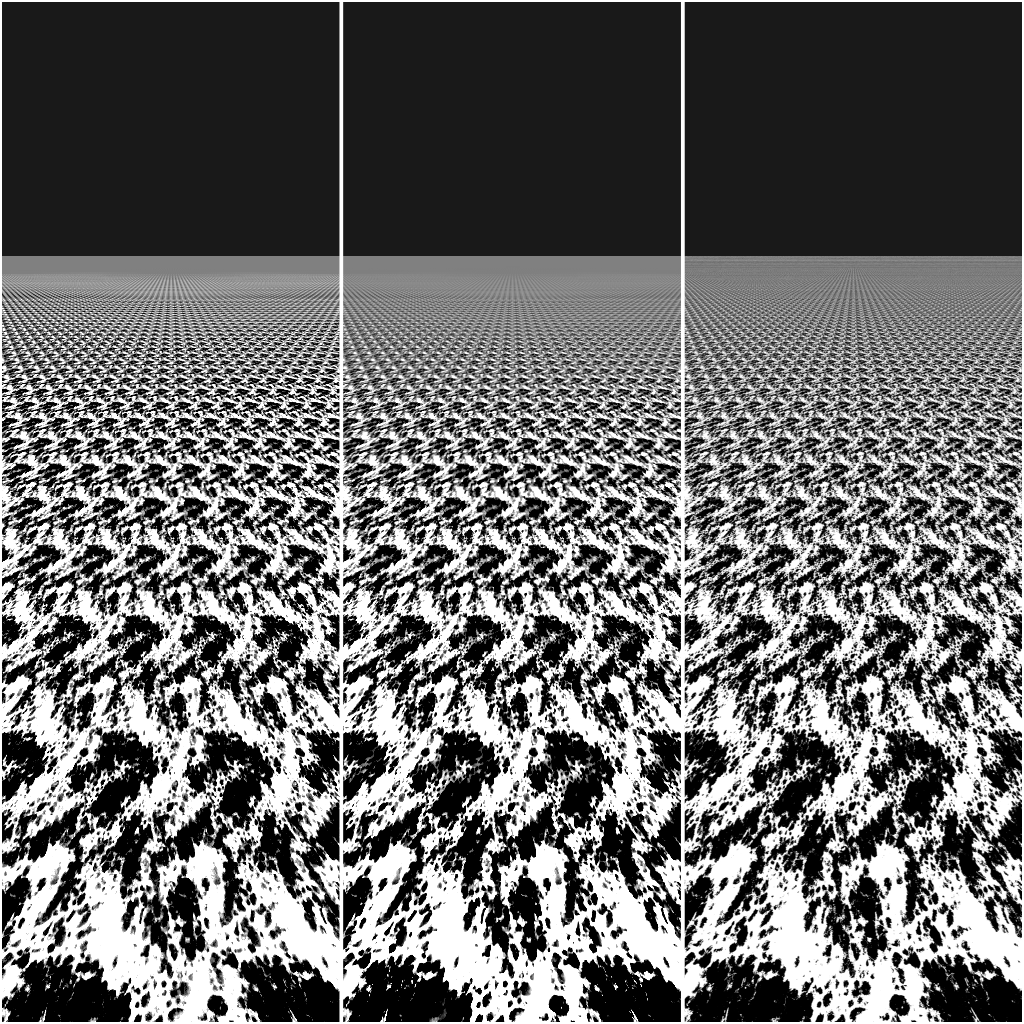
\includegraphics[width=\linewidth]{figures/MixMax/anisotrope.png}
    % \vspace{0.5em}
    \begin{minipage}{0.85\linewidth}
        \centering
        \begin{tabular}{
            >{\centering\arraybackslash}m{0.33\textwidth}
            >{\centering\arraybackslash}m{0.33\textwidth}
            >{\centering\arraybackslash}m{0.33\textwidth}
            }
            [FS24] & Ours & Ground truth \\
        \end{tabular}
    \end{minipage}

    \caption{Comparaison du filtrage anisotrope de l'influence entre la méthode [FS24], la notre et le filtrage réel de la scène. Les imprécisions sont les plus visibles à distance lointaine, sous la forme de bandes plus claires ou obscures que filtrage réel.
    }

    \label{fig::MixMax_Priority}
\end{figure}

\begin{figure}[ht]
    \centering
    \begin{tabular}{c c c}

        \subf{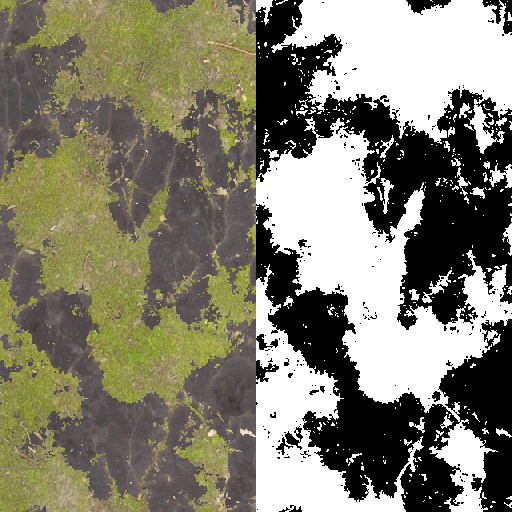
\includegraphics[width=0.15\textwidth]{figures/MixMax/Filtrage_Naif/512.png}}
        {Binary MixMax           \\ 512x512}
         &
        \subf{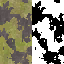
\includegraphics[width=0.15\textwidth]{figures/MixMax/Filtrage_Naif/64.png}}
        {Binary MixMax           \\ 64x64 approximation}
         &
        \subf{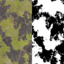
\includegraphics[width=0.15\textwidth]{figures/MixMax/Filtrage_Naif/64_ground.png}}
        {Binary MixMax           \\ 64x64 ground truth}
        \\

        \subf{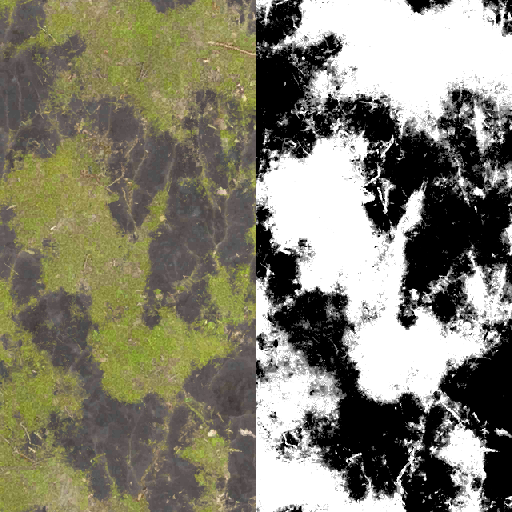
\includegraphics[width=0.15\textwidth]{figures/MixMax/Filtrage_FS24/512.png}}
        {[FS24] $\lambda = 0.01$ \\ 512x512}
         &
        \subf{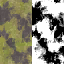
\includegraphics[width=0.15\textwidth]{figures/MixMax/Filtrage_FS24/64.png}}
        {[FS24] $\lambda = 0.01$ \\ 64x64 approximation}
         &
        \subf{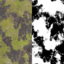
\includegraphics[width=0.15\textwidth]{figures/MixMax/Filtrage_FS24/64_ground.png}}
        {[FS24] $\lambda = 0.01$ \\ 64x64 ground truth}
        \\

        \subf{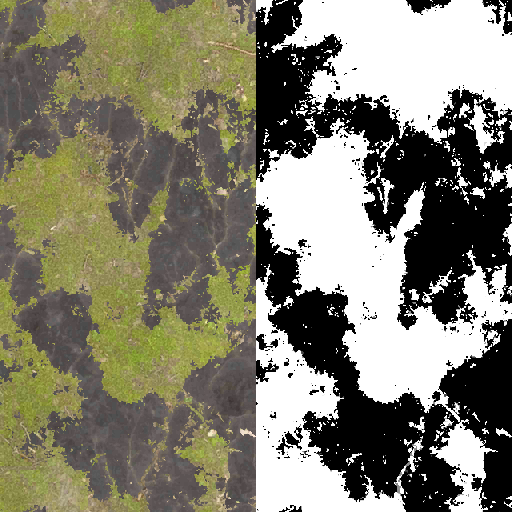
\includegraphics[width=0.15\textwidth]{figures/MixMax/Filtrage_NOUS/512.png}}
        {Ours $\lambda = 0.01$   \\ 512x512}
         &
        \subf{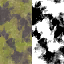
\includegraphics[width=0.15\textwidth]{figures/MixMax/Filtrage_NOUS/64.png}}
        {Ours $\lambda = 0.01$   \\ 64x64 approximation}
         &
        \subf{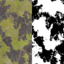
\includegraphics[width=0.15\textwidth]{figures/MixMax/Filtrage_NOUS/64_ground.png}}
        {Ours $\lambda = 0.01$   \\ 64x64 ground truth}
        \\
    \end{tabular}
    \caption{Résultat du filtrage d'une résolution de 512x512 pixels vers une résolution de 64x64. La méthode binaire, ne possédant pas de logique de filtrage, apporte une très faible qualitée à basse résolution, tandis que les méthodes utilisant la micro-priorité montrent des résultats très proche de la réalité. La principale différence entre les résultats de notre méthode et celle de [FS24] est la présence de micro-priorité visible à haute résolution. Notre méthode est ainsi identique au MixMax binaire lorsque $\lambda \rightarrow 0$.}
\end{figure}

\end{document}
